\documentclass[../main.tex]{subfiles}
\graphicspath{{\subfix{../images/}}}
\begin{document}
\section*{Term 1 Week 4}
\begin{enumerate}
    \item 
    Circle A has a radius that is \(\frac{1}{3}\) the radius of circle B. \\
    
    Starting from the position shown in the diagram, circle A rolls around circle B.\\
    
    At the end of how many revolutions of circle A will the centre of that circle first reach its starting point?\\
    \begin{figure}[h]
        \centering
        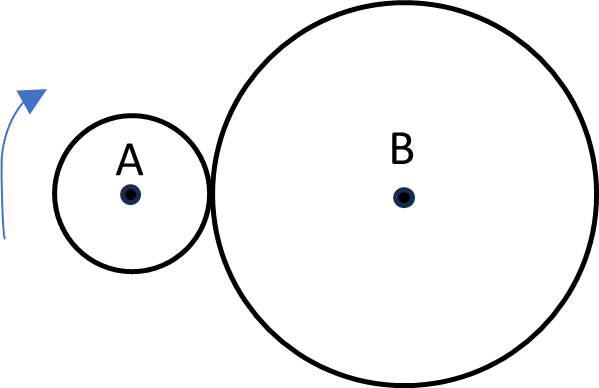
\includegraphics{images/t1w4q1.png}
    \end{figure}

    \item 
    Find the area of the red square.\\
    \begin{figure}[h]
        \centering
        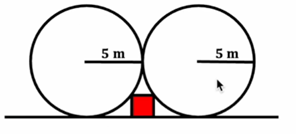
\includegraphics{images/t1w4q2.png}
    \end{figure}

    \item 
    Find the value of \(x\):\\
    \[2^x=3^{\log_5(2)}\]
\end{enumerate}

\end{document}



